\documentclass[a4paper]{article}
\usepackage[utf8]{inputenc}


%=-=-=-=-=-=-=-=-=-=-=-=-=-=-=-=-=-=-=-=-=-=-=-=-=-=-=-=-=-=-=-=-=-=-=-=-=-=-=-=-
% PREAMBLE
%=-=-=-=-=-=-=-=-=-=-=-=-=-=-=-=-=-=-=-=-=-=-=-=-=-=-=-=-=-=-=-=-=-=-=-=-=-=-=-=-

%%%%%%%%%%%%%%%%%%%%%%%%%%%%%%%%%%%%%%%%%%%%%%%%%%%%%%%%%%%%%%%%%%%%%
% Important styling notes
%%
% For now, to include img.jpg in img/path/to/img.jpg, just use:
% path/to/img.jpg - for details see style.tex
%=-=-=-=-=-=-=-=-=-=-=-=-=-=-=-=-=-=-=-=-=-=-=-=-=-=-=-=-=-=-=-=-=-=-=-=-=-=-=-=-
% Packages
%%
%\usepackage{fullpage} % Package to use full page
\usepackage[top=1in,bottom=1in,left=1in,right=1in,heightrounded]{geometry}

\usepackage{parskip}                    % Package to tweak paragraph skipping
\usepackage{amsmath}                    % standard
\usepackage{amssymb}                    % standard - Double R symbol etc.
\usepackage{hyperref}
\usepackage{amsthm}                     % standard - theorem, definition, etc.
\usepackage{multicol}                   % multiple columns for numbering
\usepackage{enumitem}                   % standard - enumerate styles
\usepackage[utf8]{inputenc}
\usepackage{scrextend}                  % indentation
\usepackage{graphicx}                   % standard - add figures
\usepackage{float}                      % standard - figure position, use [H] option
\usepackage{pifont}                     % symbols http://willbenton.com/wb-images/pifont.pdf
                                        % e.g. \ding{51}
\usepackage{gensymb}                    % degree symbol \degree
\usepackage{xcolor}                     % bg color
\hypersetup{
    colorlinks,
    linkcolor={black!50!black},
    citecolor={blue!50!black},
    urlcolor={blue!80!black}
}
\usepackage{framed}                     % bg color
\usepackage[T1]{fontenc}                % small caps
\usepackage{sectsty}                    % headings colour
\usepackage{mathtools}                  % Loads amsmath
\usepackage{amsthm,thmtools,xcolor}     % coloured theorem
\usepackage[toc,page]{appendix}         % reference to appendix
%\usepackage{titlesec}                   % change chapter, section, etc. formats
\usepackage{xifthen}                    % if, else
\usepackage{etoolbox}
% format numbering in theorem, lemma, etc. environment
\AtBeginEnvironment{theorem}{\setlist[enumerate, 1]{font=\upshape,  wide=0.5em, before=\leavevmode}}
\AtBeginEnvironment{lemma}{\setlist[enumerate, 1]{font=\upshape,  wide=0.5em, before=\leavevmode}}
\usepackage[letterspace=150]{microtype} % \textls{<letterspaced text>} % 0 <= letterspace <= 1000, 1000 = M space
\usepackage{letltxmacro}                % renew commands?
\usepackage{minted}                     % package to list code
    % otherwise minted goes off the page
    \setmintedinline{breaklines}
\usepackage{subfig}
\usepackage{eso-pic}                    % title page bg pic
\usepackage{varwidth}
\PassOptionsToPackage{svgnames}{xcolor}
\usepackage{fontawesome}                % \faQuestionCircle
\usepackage{marvosym}                   %\Pointinghand
\usepackage{mdframed}                   % easy outline frames
\usepackage[many]{tcolorbox}            % colour box for theorem styles
\usepackage{array,booktabs,calc} % table figs and text
\usepackage{comment}                    % \begin{comment}
\usepackage{fancyhdr}                   % page headings
\usepackage{mdframed}                   % boxes
\usepackage[backend=biber,sorting=none,style=ieee]{biblatex}
\usepackage{caption}
%%% caption options {
%\DeclareCaptionFont{white}{\color{white}}
\DeclareCaptionFormat{listing}{\colorbox{magenta!30!gray}{\parbox{\textwidth}{#1#2#3}}}
\captionsetup[lstlisting]{format=listing,labelfont={bf,small},textfont=small,skip=-1pt}
%%% }
\addbibresource{bibliography.bib}
\usepackage{url}
\usepackage{textcomp}
\usepackage[makeroom]{cancel}           % crossed symbols - \cancel{}, \bcancel{}, xcancel{}
\usepackage{algorithm}
\usepackage[noend]{algpseudocode}
\usepackage{tikz}
\usetikzlibrary{arrows.meta,positioning,quotes} % arrows and nodes in tikz
\usepackage{marginnote}                 % things in page margin by \marginnote{...}
\usepackage{pgfplots}
\usepackage{pstricks-add,pst-slpe}      % for fancy tikz arrows
%\usepackage{titlesec}                  % title style
\usepackage{lmodern}                    % a font
\usepackage{titletoc}                   % Required for manipulating the table of contents
\usepackage{titlesec}                   % Allows customization of titles
\usepackage{fouriernc}                  % Use the New Century Schoolbook font
\usepackage{booktabs}                   % better tables
\usepackage{stmaryrd }                  % \varoast
\usepackage{listings}                   % code listings
\usepackage{longtable}                  % table across multiple pages
\usepackage{todonotes}                  % TODO bubbles by \todo{...} command
\usepackage{changepage}                 % paragraph margins
\usepackage{tikz}
\usetikzlibrary{calc}
\usepackage{eso-pic}
\usepackage{transparent}



%=-=-=-=-=-=-=-=-=-=-=-=-=-=-=-=-=-=-=-=-=-=-=-=-=-=-=-=-=-=-=-=-=-=-=-=-=-=-=-=-
% Colours for various things
%%


\definecolor{shadecolor}{rgb}{1.,0.933,0.96} % bg color, r,g,b <= 1
\definecolor{medium_blue}{RGB}{60,125,190}
\definecolor{dark_blue}{RGB}{25,60,85}
\definecolor{dark_red}{RGB}{77,16,16}
\definecolor{LightPink}{rgb}{0.92.,0.8,0.84} % bg color, r,g,b <= 1
\definecolor{LighterPink}{rgb}{1.,0.94,0.97} % bg color, r,g,b <= 1
\definecolor{LightestPink}{rgb}{1.,0.95,0.99} % bg color, r,g,b <= 1
\definecolor{DarkestPink}{rgb}{0.36, 0.0, 0.18}
\definecolor{DarkerPink}{rgb}{0.41, 0.0, 0.21}
\definecolor{DarkPink}{rgb}{0.55, 0.05, 0.37}
\definecolor{lightestestpink}{RGB}{255,248,252}
\definecolor{codegray}{rgb}{0.5,0.5,0.5}
\definecolor{codegrayblue}{rgb}{0.35,0.35,0.47}



%=-=-=-=-=-=-=-=-=-=-=-=-=-=-=-=-=-=-=-=-=-=-=-=-=-=-=-=-=-=-=-=-=-=-=-=-=-=-=-=-
% Define my own theorem styles
%%

% "base" styles
\declaretheoremstyle[
  headfont=\color{DarkPink}\bfseries,
  bodyfont=\itshape,
]{colored}

\declaretheoremstyle[
  headfont=\color{DarkPink}\bfseries,
  bodyfont=\normalfont,
]{colored_upright}

% theorems (corollaries, etc) themselves, inherit from my style above
% Usage:
% \begin{theorem} \end{theorem}, \begin{lemma} \end{lemma}, ...
\declaretheorem[
	numberwithin=section,
 	style=colored,
	name=\textsc{Theorem},
]{theorem}

\tcolorboxenvironment{theorem}{
  boxrule=0pt,
  boxsep=2pt,
  colback={magenta!25!white},
  colframe=DarkPink,
  enhanced jigsaw, 
  borderline west={2pt}{0pt}{DarkPink},
  sharp corners,
  before skip=5pt,
  after skip=5pt,
  breakable,
  right=0mm % for equations
}

\declaretheorem[
	numberwithin=section,
 	style=colored,
	name=\textsc{Corollary},
]{corollary}

\tcolorboxenvironment{corollary}{
  boxrule=0pt,
  boxsep=1pt,
  colback={magenta!10!white},
  colframe=DarkPink,
  enhanced jigsaw, 
  borderline west={2pt}{0pt}{DarkPink},
  sharp corners,
  before skip=5pt,
  after skip=5pt,
  breakable,
  right=0mm % for equations
}

\declaretheorem[
	numberwithin=section,
	style=colored,
	name=\textsc{Lemma},
]{lemma}

\tcolorboxenvironment{lemma}{
  boxrule=0pt,
  boxsep=1pt,
  colback={magenta!10!white},
  colframe=DarkPink,
  enhanced jigsaw, 
  borderline west={2pt}{0pt}{DarkPink},
  sharp corners,
  before skip=5pt,
  after skip=5pt,
  breakable,
  right=0mm % for equations
}

\declaretheorem[
	numberwithin=section,
	style=colored,
	name=\textsc{Definition},
]{definition}

\tcolorboxenvironment{definition}{
  boxrule=0pt,
  boxsep=1pt,
  colback={magenta!25!white},
  colframe=DarkPink,
  enhanced jigsaw, 
  borderline west={2pt}{0pt}{DarkPink},
  sharp corners,
  before skip=5pt,
  after skip=5pt,
  breakable,
  right=0mm % for equations
}

\declaretheorem[
	numberwithin=section,
  	style=colored,
  	name=\textsc{Example},
]{exmp}

\declaretheorem[
	numberwithin=section,
  	style=colored,
  	name=\textsc{Solution},
]{soln}

%%% code listings
\lstdefinestyle{code1}{
    backgroundcolor=\color{lightestestpink},   
    commentstyle=\color{codegrayblue},
    keywordstyle=\color{DarkerPink},
    numberstyle=\tiny\color{codegray},
    stringstyle=\color{black!40!cyan},
    basicstyle=\small\ttfamily,
    breakatwhitespace=false,
    breaklines=true,        
    captionpos=t,             
    keepspaces=true,        
    numbers=left,           
    numbersep=5pt,
    showspaces=false, 
    showstringspaces=false,
    showtabs=false,
    tabsize=4
}

%%% code listings
\lstdefinestyle{code1}{
    backgroundcolor=\color{lightestestpink},   
    commentstyle=\color{codegrayblue},
    keywordstyle=\color{DarkerPink},
    numberstyle=\tiny\color{codegray},
    stringstyle=\color{black!40!cyan},
    basicstyle=\small\ttfamily,
    breakatwhitespace=false,
    breaklines=true,        
    captionpos=t,             
    keepspaces=true,        
    numbers=left,           
    numbersep=5pt,
    showspaces=false, 
    showstringspaces=false,
    showtabs=false,
    tabsize=4
}


\lstdefinestyle{terminal}{
    backgroundcolor=\color{black!5},   
    commentstyle=\color{codegrayblue},
    keywordstyle=\color{DarkerPink},
    %numberstyle=\tiny\color{codegray},
    stringstyle=\color{black!40!cyan},
    basicstyle=\small\ttfamily,
    numbers=none,
    breakatwhitespace=false,
    breaklines=true,        
    %captionpos=t,             
    keepspaces=true,        
    %numbers=left,           
    %numbersep=5pt,
    showspaces=false, 
    showstringspaces=false,
    showtabs=false,
    tabsize=4
}

\lstset{style=code1}

%=-=-=-=-=-=-=-=-=-=-=-=-=-=-=-=-=-=-=-=-=-=-=-=-=-=-=-=-=-=-=-=-=-=-=-=-=-=-=-=-
% Headers (size, font, colour)
%%

\makeatletter
\renewcommand{\@seccntformat}[1]{\llap{\textcolor{DarkestPink}{\csname the#1\endcsname}\hspace{1em}}}                    
\renewcommand{\section}{\@startsection{section}{1}{\z@}
{-4ex \@plus -1ex \@minus -.4ex}
{1ex \@plus.2ex }
{\normalfont\large\sffamily\bfseries\textcolor{DarkestPink}}}
\renewcommand{\subsection}{\@startsection {subsection}{2}{\z@}
{-3ex \@plus -0.1ex \@minus -.4ex}
{0.5ex \@plus.2ex }
{\normalfont\sffamily\bfseries\textcolor{DarkestPink}}}
\renewcommand{\subsubsection}{\@startsection {subsubsection}{3}{\z@}
{-2ex \@plus -0.1ex \@minus -.2ex}
{.2ex \@plus.2ex }
{\normalfont\small\sffamily\bfseries\textcolor{DarkestPink}}}                        


%=-=-=-=-=-=-=-=-=-=-=-=-=-=-=-=-=-=-=-=-=-=-=-=-=-=-=-=-=-=-=-=-=-=-=-=-=-=-=-=-
% Numberings, counters and spacings
%%
\numberwithin{equation}{section} % section number in eq/s
\setlength{\jot}{7pt} % spacing in split, gathered env/s



%% Custom examples
%% Output - Example 1,2,...
\newcounter{example}
\newenvironment{example}[1][]{\refstepcounter{example}\par\medskip
   \textbf{Example~\theexample. #1} \rmfamily}{\medskip}
%%%%%%%%%%%% End of unused %%%%%%%%%%%%



%=-=-=-=-=-=-=-=-=-=-=-=-=-=-=-=-=-=-=-=-=-=-=-=-=-=-=-=-=-=-=-=-=-=-=-=-=-=-=-=-
% Paths
%%

%=-=-=-=-=-=-=-=-=-=-=-=-=-=-=-=-=-=-=-=-=-=-=-=-=-=-=-=-=-=-=-=-=-=-=-=-=-=-=-=-
% User defined macros (math mode)
%%


% Curly braces under text. Usage: \myunderbrace{upper}{lower}
\newcommand{\myunderbrace}[2]{\mathrlap{\underbrace{\phantom{#1}}_{#2}} #1}
\newcommand{\setR}{\mathbb{R}} % \ouble R
\newcommand{\setRn}{\mathbb{R}^n} %  double R^n
\newcommand{\setN}{\mathbb{N}} % double N
\newcommand{\setZ}{\mathbb{Z}} % double Z
\let\oldemptyset\emptyset
\let\emptyset\varnothing % nice - looking empty set symbol
\newcommand{\fancyN}{\mathcal{N}} % null space
\newcommand{\fancyR}{\mathcal{R}} % range

\newcommand{\ba}{\textbf{a}}
\newcommand{\bw}{\textbf{w}}
\newcommand{\bx}{\textbf{x}}
\newcommand{\bu}{\textbf{u}}
\newcommand{\by}{\textbf{y}}
\newcommand{\bz}{\textbf{z}}
\newcommand{\bb}{\textbf{b}}
\newcommand{\bA}{\textbf{A}}
\newcommand{\bB}{\textbf{B}}
\newcommand{\bC}{\textbf{C}}
\newcommand{\bD}{\textbf{C}}
\newcommand{\bI}{\textbf{I}}
\newcommand{\bO}{\textbf{0}}
\newcommand{\bS}{\textbf{S}}
\newcommand{\bX}{\textbf{X}}
\newcommand{\bU}{\textbf{U}}
\newcommand{\bY}{\textbf{Y}}
% double bars as in norm
%\newcommand{\norm}[1] {\left|\left| #1 \right| \right|} 
\newcommand{\norm}[1]{\left\lVert#1\right\rVert}
\renewcommand{\t}{^{\top}}

\newcommand{\mean}[1]{\bar{#1}}
\newcommand{\var}{\sigma^2}

\newcommand{\partdevx}[1]{\frac{\partial #1}{\partial x}}
\newcommand{\partdevt}[1]{\frac{\partial #1}{\partial t}}
\newcommand{\partdevxx}[1]{\frac{\partial #1}{\partial x}}
\newcommand{\partdevxn}[1]{\frac{\partial^n #1}{\partial x^n}}
\newcommand{\partdevy}[1]{\frac{\partial #1}{\partial y}}
\newcommand{\partdevyy}[1]{\frac{\partial #1}{\partial y}}
\newcommand{\partdevyn}[1]{\frac{\partial^n #1}{\partial y^n}}

% text above = symbol
\newcommand{\overeq}[1]{\ensuremath{\stackrel{#1}=}} 
\newcommand{\greatersmaller}{%
  \mathrel{\ooalign{\raisebox{.6ex}{$>$}\cr\raisebox{-.6ex}{$<$}}}
} % greater and smaller symbols on top of each other, same line

%=-=-=-=-=-=-=-=-=-=-=-=-=-=-=-=-=-=-=-=-=-=-=-=-=-=-=-=-=-=-=-=-=-=-=-=-=-=-=-=-
% User defined macros (non math)

\newcommand{\qedblack}{$\hfill\blacksquare$} % black square end of line
\newcommand{\qedwhite}{\hfill \ensuremath{\Box}} % white square end of line
\newcommand{\hquad}{\hskip0.5em\relax}% half quad space
%\newcommand{\TODO}{\textcolor{red}{\bf TODO!}\;}

\newcommand{\TODO}[1][]{%
    \ifthenelse{\equal{#1}{}}{\textcolor{red}{\bf TODO!}\;}{\textcolor{red}{\textbf {TODO:} #1}\; }%
}
\newcommand{\B}[1]{\textbf{\textup{#1}}} % bold and upright
\renewcommand{\labelitemi}{\scriptsize$\textcolor{DarkPink}{\blacksquare}$} % itemize - squares instead of bullets
\newcommand{\emphasis}[1]{\textls{#1}}

\LetLtxMacro{\originaleqref}{\eqref}
\renewcommand{\eqref}{Eq.~\originaleqref}
\renewcommand*{\eqref}[1]{Eq.~\originaleqref{#1}}





% background images
%%%%%%%
\newcommand\BackgroundPic{%
\put(0,0){%
\parbox[b][\paperheight]{\paperwidth}{%
\vfill
%\centering
\includegraphics[width=0.125\paperwidth,height=\paperheight,%
]{img/background_02.png}% use ,keepaspectratio
\vfill
}}}
%%%%%%%
% end of background image
%%%%%%%%%%%%%% my own frame
\newmdenv[topline=false,bottomline=false]{leftrightbox}
%%%%%%%%%%%%% end
%%%%%%%%%%%%% my own comment
\newcommand{\mycomment}[1]{\begin{leftrightbox}\Pointinghand~\textbf{Comment:}~#1 \end{leftrightbox}}
%%%%%%%%%%%%% end
% my custom note https://tex.stackexchange.com/questions/301993/create-custom-note-environment-with-tcolorbox
\newmdenv[
    topline=false,
    bottomline=false,
    rightline=false,
    innerrightmargin=0pt
]{siderule}
\newenvironment{mynote}%
    {\begin{siderule}\textbf{\Pointinghand~Note:}}
    {\end{siderule}}
    
\newenvironment{myquote}%
    {\begin{adjustwidth}{0.4cm}{0.4cm}\faQuoteLeft\ \itshape}
    { \hfill \faQuoteRight  \end{adjustwidth}}
%%%%%%%%%%%%% my own box
\newcommand{\boxone}[1]{\begin{tcolorbox}[colback = LighterPink,colframe=LightPink]
#1
\end{tcolorbox}}
%%%%%%%%%%%%% end

\let\oldemptyset\emptyset
\let\emptyset\varnothing
%algorithmic
\algdef{SE}[DOWHILE]{Do}{doWhile}{\algorithmicdo}[1]{\algorithmicwhile\ #1}%

%%% otherwise minted goes off the page
\setmintedinline{breaklines}





\begin{document}
%=-=-=-=-=-=-=-=-=-=-=-=-=-=-=-=-=-=-=-=-=-=-=-=-=-=-=-=-=-=-=-=-=-=-=-=-=-=-=-=-
% GLOBAL STYLES (DOCUMENT SCOPE)
%=-=-=-=-=-=-=-=-=-=-=-=-=-=-=-=-=-=-=-=-=-=-=-=-=-=-=-=-=-=-=-=-=-=-=-=-=-=-=-=-
% caption: Figure 1 -> <bold> Fig. 1 </bold>
\captionsetup[figure]{labelfont={bf},labelformat={default},labelsep=period,name={Fig.}}


%=-=-=-=-=-=-=-=-=-=-=-=-=-=-=-=-=-=-=-=-=-=-=-=-=-=-=-=-=-=-=-=-=-=-=-=-=-=-=-=-
% TITLE PAGE
%=-=-=-=-=-=-=-=-=-=-=-=-=-=-=-=-=-=-=-=-=-=-=-=-=-=-=-=-=-=-=-=-=-=-=-=-=-=-=-=-
%%%%%%%%%%%%%%%%%%%%%%%%%%%%%%%%%%%%%%%%%
% Formal Book Title Page
% LaTeX Template
% Version 2.0 (23/7/17)
%
% This template was downloaded from:
% http://www.LaTeXTemplates.com
%
% Original author:
% Peter Wilson (herries.press@earthlink.net) with modifications by:
% Vel (vel@latextemplates.com)
%
% License:
% CC BY-NC-SA 3.0 (http://creativecommons.org/licenses/by-nc-sa/3.0/)
% 
% This template can be used in one of two ways:
%
% 1) Content can be added at the end of this file just before the \end{document}
% to use this title page as the starting point for your document.
%
% 2) Alternatively, if you already have a document which you wish to add this
% title page to, copy everything between the \begin{document} and
% \end{document} and paste it where you would like the title page in your
% document. You will then need to insert the packages and document 
% configurations into your document carefully making sure you are not loading
% the same package twice and that there are no clashes.
%
%%%%%%%%%%%%%%%%%%%%%%%%%%%%%%%%%%%%%%%%%

%----------------------------------------------------------------------------------------
%	PACKAGES AND OTHER DOCUMENT CONFIGURATIONS
%----------------------------------------------------------------------------------------



%----------------------------------------------------------------------------------------
%	TITLE PAGE
%----------------------------------------------------------------------------------------



\begin{titlepage} % Suppresses headers and footers on the title page

    
   	%------------------------------------------------
	%	Text alignment
	%------------------------------------------------
	\centering % Centre everything on the title page
	
	\scshape % Use small caps for all text on the title page
	
	\vspace*{\baselineskip} % White space at the top of the page
	
	%------------------------------------------------
	%	Title
	%------------------------------------------------
	
	\rule{\textwidth}{1.6pt}\vspace*{-\baselineskip}\vspace*{2pt} % Thick horizontal rule
	\rule{\textwidth}{0.4pt} % Thin horizontal rule
	
	\vspace{0.75\baselineskip} % Whitespace above the title
	
	{\LARGE SHAPE RASTERISATION\\ \Large ALGORITHMS\\} % Title
	
	\vspace{0.75\baselineskip} % Whitespace below the title
	
	\rule{\textwidth}{0.4pt}\vspace*{-\baselineskip}\vspace{3.2pt} % Thin horizontal rule
	\rule{\textwidth}{1.6pt} % Thick horizontal rule
	
	\vspace{2\baselineskip} % Whitespace after the title block
	
	%------------------------------------------------
	%	Subtitle
	%------------------------------------------------
        Contents
	
	\vspace*{3\baselineskip} % Whitespace under the subtitle
	
        Straight Lines\\
        Curvy Lines\\
        Triangle Fill\\
        Circle Drawing
	
	\vspace*{3\baselineskip} % Whitespace under the subtitle
	
	%------------------------------------------------
	%	Editor(s)
	%------------------------------------------------
	
	By
	
	\vspace{0.5\baselineskip} % Whitespace before the editors
	
	{\normalfont \Large \mintinline{latex}{0xLeo} (\url{github.com/0xleo}) \\} % Editor list
	
	\vspace{0.5\baselineskip} % Whitespace below the editor list
	
	%\textit{The University of California \\ Berkeley} % Editor affiliation
	
	\vfill % Whitespace between editor names and publisher logo
	
	%------------------------------------------------
	%	Publisher
	%------------------------------------------------
	
	
	\vspace{0.3\baselineskip} % Whitespace under the publisher logo
	
	\today % Date
	
	{DRAFT X.YY} % Draft version
	{\\Missing: \ldots}

\end{titlepage}

%----------------------------------------------------------------------------------------

%\maketitle



%=-=-=-=-=-=-=-=-=-=-=-=-=-=-=-=-=-=-=-=-=-=-=-=-=-=-=-=-=-=-=-=-=-=-=-=-=-=-=-=-
% MAIN DOCUMENT
%=-=-=-=-=-=-=-=-=-=-=-=-=-=-=-=-=-=-=-=-=-=-=-=-=-=-=-=-=-=-=-=-=-=-=-=-=-=-=-=-
\newpage
\tableofcontents
\newpage



%------------------------------ New section ------------------------------%
\section{UML class diagrams}

\subsection{Class representation}
In Object-Oriented Programming (OOP), Unified Modeling Language (UML) class diagram is a notation to visualise classes, their data, operations and the relationships between them. A class is visualised with a rectangle while relationships are visualised by arrows.

Classes are visualised as boxes, with their public data and methods preceeded by \texttt{+} and their private ones by \texttt{-}. In Fig. \ref{fig:atm_uml}, the ATM class has the \texttt{deposit(int amount), withdraw(int amount)} as public methods and \texttt{cash} as private data.

\begin{figure}[ht]
  \centering
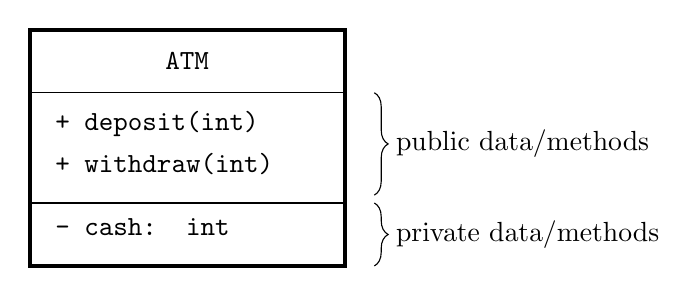
\begin{tikzpicture}
  % Class Rectangle
  \draw[line width=1.5pt] (0,1) rectangle (4,4);
  % Class Title
  \node[align=center] at (2,3.6) {\texttt{ATM}};
  % Public Methods Section
  \draw (0,3.2) -- (4,3.2);
  \node[align=left,anchor=west] at (0.2,2.8) {\texttt{+ deposit(int)}};
  \node[align=left,anchor=west] at (0.2,2.3) {\texttt{+ withdraw(int)}};
  \draw[decorate, decoration={brace, amplitude=5pt,  raise=5pt}]
  (4.2,3.2) -- (4.2,1.9) node[midway, right=6pt, align=center] {\,\,public data/methods};

  % Private Data Section
  \draw (0,1.8) -- (4,1.8);
  \node[align=left,anchor=west] at (0.2,1.5) {\texttt{- cash: int}};
  \draw[decorate, decoration={brace, amplitude=5pt,  raise=5pt}]
  (4.2,1.8) -- (4.2,1) node[midway, right=6pt, align=center] {\,\,private data/methods};
\end{tikzpicture}
\caption{UML block of a simplified ATM class.}
\label{fig:atm_uml}
\end{figure}


\subsection{UML arrows}

A and B denote two class instances. So normally they would be represented by boxes but for brevity they're represented by letters.
    \begin{longtable}{p{0.2\textwidth} p{0.2\textwidth} p{0.6\textwidth}}
        \hline
        \textbf{Arrow} & \textbf{Name and explanation} & \textbf{C++ example} \\
        \hline
        %----- Column 1 -----
        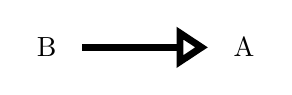
\begin{tikzpicture}
        \draw[-{Triangle[open, fill=white, length=4mm, width=5mm]}, line width=2.5pt] (0.2,2) -- (1.8,2);
        \node[anchor=east] at (0,2) {B};
        \node[anchor=west] at (2,2) {A};
        \end{tikzpicture} &
        %----- Column 2 -----
        \textit{Inheritance}

        B inherits from A, i.e. it inherits its public/private methods and data including their implementation. B is free to overwrite their implementation.
        &
        %----- Column 3 -----
        \begin{minted}[]{cpp}
class A {
public:
  // will be inherited
  int foo() { return 42; }
protected:
  // will be inherited
  unsigned bar() { return 1337; }
private:
  // will not be inherited
};

class B: public A {
public:
  unsigned bar() { return 0xdeadbeef; }
};

int main()
{
  B b;
  b.foo(); // 42
  b.bar(); // 0xdeadbeef
}
        \end{minted}
        \\
        \hline

        %----- Row 2 ----
        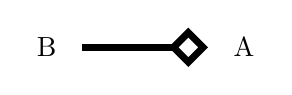
\begin{tikzpicture}
            \draw[-{Diamond[open, fill=white, length=5mm,   width=5mm]}, line width=2.5pt] (0.2,2) -- (1.8,2);
            \node[anchor=east] at (0,2) {B};
            \node[anchor=west] at (2,2) {A};
        \end{tikzpicture} &
        \textit{(Weak) aggregation}

        B is associated with A but B's lifetime does not necessarily depend on A's -- if B is destroyed, A may still live.

        Summary: B has but shares an object B.
        &
        \begin{minted}[]{cpp}
#include <iostream>

class B
{
public:
  ~B() { std::cout << "B is destroyed\n"; }
};

class A
{
public:
  A(): obj(nullptr) {};
  ~A() { std::cout << "A is destroyed\n"; }
  void SetB(const B& b) { *obj = b; }
private:
  B* obj;
};
        \end{minted} 
        \\

        % ---------------- Row ----------------
        &
        
        
        &
        \begin{minted}[]{cpp}
#include <iostream>
class A {
public:
  ~A() { std::cout << "A is destroyed\n"; }
};

class B {
public:
  B(): obj(nullptr) {};
  ~B() { std::cout << "B is destroyed\n"; }
void SetA(const A& a) { *obj = a; }
private:
  A* obj;
};

int main() {
  A a;
  bool do_something = true;
  if (do_something) {
    B b;
    b.SetA(a);
  }
  // a is still alive
}
        \end{minted} 
        \\
        \hline

        % ---------------- Row ----------------
        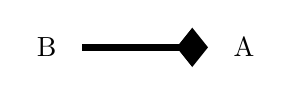
\begin{tikzpicture}
            \draw[-{Diamond[open, fill=black, length=4mm,   width=5mm]}, line width=2.5pt] (0.2,2) -- (1.8,2);
            \node[anchor=east] at (0,2) {B};
            \node[anchor=west] at (2,2) {A};
        \end{tikzpicture}
        &
        \textit{Strong aggregation} aka \textit{composition}.

        B fully contains A. Composition occurs when a class contains another one as part and lifetime of contained object (A) is tightly bound to the lifetime of the container (B).

        Summary: B has and owns an object A.
        
        &
        \begin{minted}[]{cpp}
#include <iostream>

class A {
public:
  A() { std::cout << "A is created\n"; }
  ~A() { std::cout << "A is destroyed\n"; }
  void foo() { std::cout << "A is calling foo\n"; }
};

class B {
public:
  B() { std::cout << "B is created\n"; }
  ~B() { std::cout << "B is destroyed\n"; }
  A a;
private:
};

int main()
{
  B b;
  b.a.foo(); // a exists only within b
}
        \end{minted} 
        \\
        \hline

        % ---------------- Row ----------------
        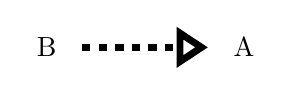
\begin{tikzpicture}
            \draw[-{Triangle[open, fill=white, length=4mm,   width=5mm]}, dashed, line width=2.5pt] (0.2,2) -- (1.8,2);
            \node[anchor=east] at (0,2) {B};
            \node[anchor=west] at (2,2) {A};
        \end{tikzpicture}
        &
        \textit{Realisation}.

        B realises A. In this case, A is an interface; it defines but does not implement its methods. A's methods are called abstract. B inherits from it and implements its methods.
        &
        \begin{minted}[]{cpp}
#include <iostream>

// interface class
class A {
public:
  // abstract (aka virtual) unimplemented methods
  virtual int foo() = 0;
  virtual int bar() = 0;
};
        \end{minted} 
        \\

        % ---------------- Row ----------------
        &
 
        &
        \begin{minted}[]{cpp}
// inherit A and then implement all its methods
class B: public A {
public:
  // implement abstract methods (virtual->override)
  int foo() override { return 42; }
  int bar() override { return 1337; }
};

int main() {
  B b;
  std::cout << b.foo() << std::endl;
  std::cout << b.bar() << std::endl;
}
        \end{minted} 
        \\
        \hline

        % ---------------- Row ----------------
        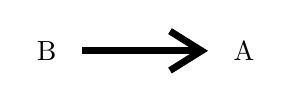
\begin{tikzpicture}
            \draw[-{Straight Barb[open, fill=white, length=4mm, width=5mm]}, line width=2.5pt] (0.2,2) -- (1.8,2);

            \node[anchor=east] at (0,2) {B};
            \node[anchor=west] at (2,2) {A};
        \end{tikzpicture}
        &
        \textit{Association}

        Class B has a connection to class A.
        
        Association is a broad term to represent the ``has-a'' relationship between two classes. It means that an object of one class somehow communicates to an object of another.

        Summary: B has an object A.
        &
        \begin{minted}[]{cpp}
class A {
public:
  int foo() { return 420; }
};

class B {
public:
  B(A& a): a_(a) {};
  int bar() { return a_.foo(); }
private:
    A& a_; // has-a reference
};

int main() {
  A a;
  B b(a);
  b.bar(); // a.foo()
}
        \end{minted} 
        \\
        \hline

    \caption{UML class diagram arrow meanings.} \label{tab:uml_arrows_table}
\end{longtable}

For example, the relationship of a shirt having a pocket is composition since a pocket only exists in a shirt but the relationship of a car having a wheel is aggregation as a wheel can be removed and used by another car.

\begin{figure}[ht]
  \centering
  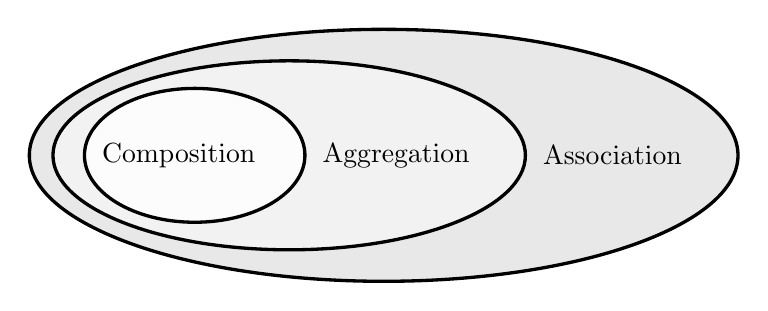
\begin{tikzpicture}
    \filldraw[fill=gray!18, very thick] (3.9,0) ellipse (4.5 and 1.6);
    \filldraw[fill=gray!10, very thick] (2.7,0) ellipse (3 and 1.2);
    \filldraw[fill=gray!2, very thick] (1.5,0) ellipse (1.4 and 0.85);
    \node[align=left,anchor=west] at (0.2,0) {Composition};
    \node[align=left,anchor=west] at (3,0) {Aggregation};
    \node[align=left,anchor=west] at (5.8,0) {Association};
  \end{tikzpicture}
  \caption{Superset view of the ``has-a'' OOP relationships.} \label{fig:oop_hasa_superset}
\end{figure}


\subsection{Abstract Class vs Interface}

\textit{Interface} and \textit{abstract class} are two terms to define classes that have at least one \textit{pure virtual method} (aka \textit{abstract method}), i.e. one unimplemented method meant to be implemented by a subclass. In C++, pure (virtual) methods are denoted by the following syntax:
\begin{verbatim}
virtual void MyAbstractMethod(int i) = 0;
\end{verbatim}

The difference is that an interface ONLY contains abstract methods while an abstract class is simply one with at least one abstract method and is allowed to contain its own implemented (non-virtual) methods as well.

\begin{table}[H]
  \centering
  \begin{tabular}{p{0.45\linewidth}|p{0.45\linewidth}}
    \textbf{Interface} & \textbf{Abstract class} \\
    \hline
        \begin{minted}[]{cpp}
class Interface {
public:
  // virtual destructor to ensure
  // proper deletion
  virtual ~Interface() {};
  virtual void AbstractMethod1() = 0;
  virtual void AbstractMethod2() = 0;
};
        \end{minted}
        &
        \begin{minted}[]{cpp}
class AbstractClass {
public:
  // virtual destructor
  virtual ~Interface() {};
  virtual void AbstractMethod1() = 0;
  virtual void AbstractMethod2() = 0;
  int Method1(int i);
};
        \end{minted}
        \\
    \hline
  \end{tabular}
  \caption{The difference between interface and abstract class in C++.}
  \label{tab:interface_vs_abstract_class}
\end{table}

\section{Software Design Patterns}

A design pattern is a tried and true solution to a common problem. Particularly, they provide standard OOP solutions to common problems while making components of the system reusable. 


\subsection{The 23 Gang of Four Design Patterns}

\textit{Creational patterns} deal with object creation mechanisms, \textit{structural patterns} ease the design by identifying a simple way to realise
relationships between entities and \textit{behavioural patterns} are concerned with communication between objects. There exist 23 established design patterns listed in Table \ref{tab:gang_of_four_23}.

\begin{table}[H]
  \centering
  \begin{tabular}{p{0.3\linewidth}|p{0.3\linewidth}|p{0.3\linewidth}}
    \textbf{Creational} & \textbf{Structural} & \textbf{Behavioural} \\
    \midrule
    Factory          & Adapter   & Interpreter  \\
    Abstract factory & Bridge    & Template method \\
    Builder          & Composite & Chain of responsibility \\
    Prototype        & Decorator & Command \\
    Singleton        & Facade    & Iterator \\
                     & Flyweight & Mediator \\
                     & Proxy     & Memento \\
                     &           & Observer \\
                     &           & State \\
                     &           & Strategy \\
                     &           & Visitor \\
    \hline
  \end{tabular}
  \caption{The "Gang of 4" 23 fundamental design patterns.}
  \label{tab:gang_of_four_23}
\end{table}

\subsubsection{Observer}

The aim of the observer pattern is to propagate state changes of the object to be observed (subject) into multiple observer objects. It does this by calling each update method of its observers. 

For example in a program to monitor stocks where the subject stores a list of stock prices. Implementing the graph view and the tabular view inside the subject itself would make it cluttered and hard to maintain. Therefore it's better to assign the responsibility of observing the price to some UI and tabular view classes and whenever the price changes they're updated.

More formally, we say that the observer pattern defines a one-to-many relationship so that when an object changes all its dependents are notified automatically when the state of the subject changes.

\begin{table}[H]
  \centering
  \begin{tabular}{p{0.25\linewidth} p{0.675\linewidth}}
\begin{minipage}[t]{\linewidth}
   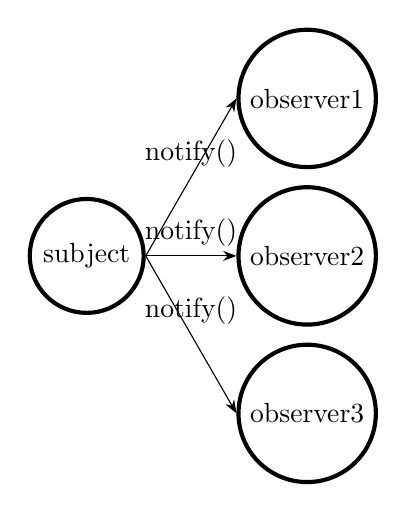
\begin{tikzpicture}[>=Stealth, node distance=2cm] 
    % Observer
    \node[circle, draw, align=center, line width=1.5pt] (subject) at (0, 0) {subject};

    \def\discm{2};
    % Subjects
    \node[circle, draw, align=center, line width=1.5pt] (observer1) at (2.8, \discm) {observer1};
    \node[circle, draw, align=center, line width=1.5pt] (observer2) at (2.8, 0) {observer2};
    \node[circle, draw, align=center, line width=1.5pt] (observer3) at (2.8, -\discm) {observer3};

    % Arrows
    \draw[->] (subject.east) -- (observer1.west) node[midway, above] {notify()};
    \draw[->] (subject.east) -- (observer2.west) node[midway, above] {notify()};
    \draw[->] (subject.east) -- (observer3.west) node[midway, above] {notify()};
\end{tikzpicture}
\captionof{figure}{The observer pattern describes and one-to-many relationship.}
\end{minipage}

  & \begin{minipage}[t]{\linewidth}
    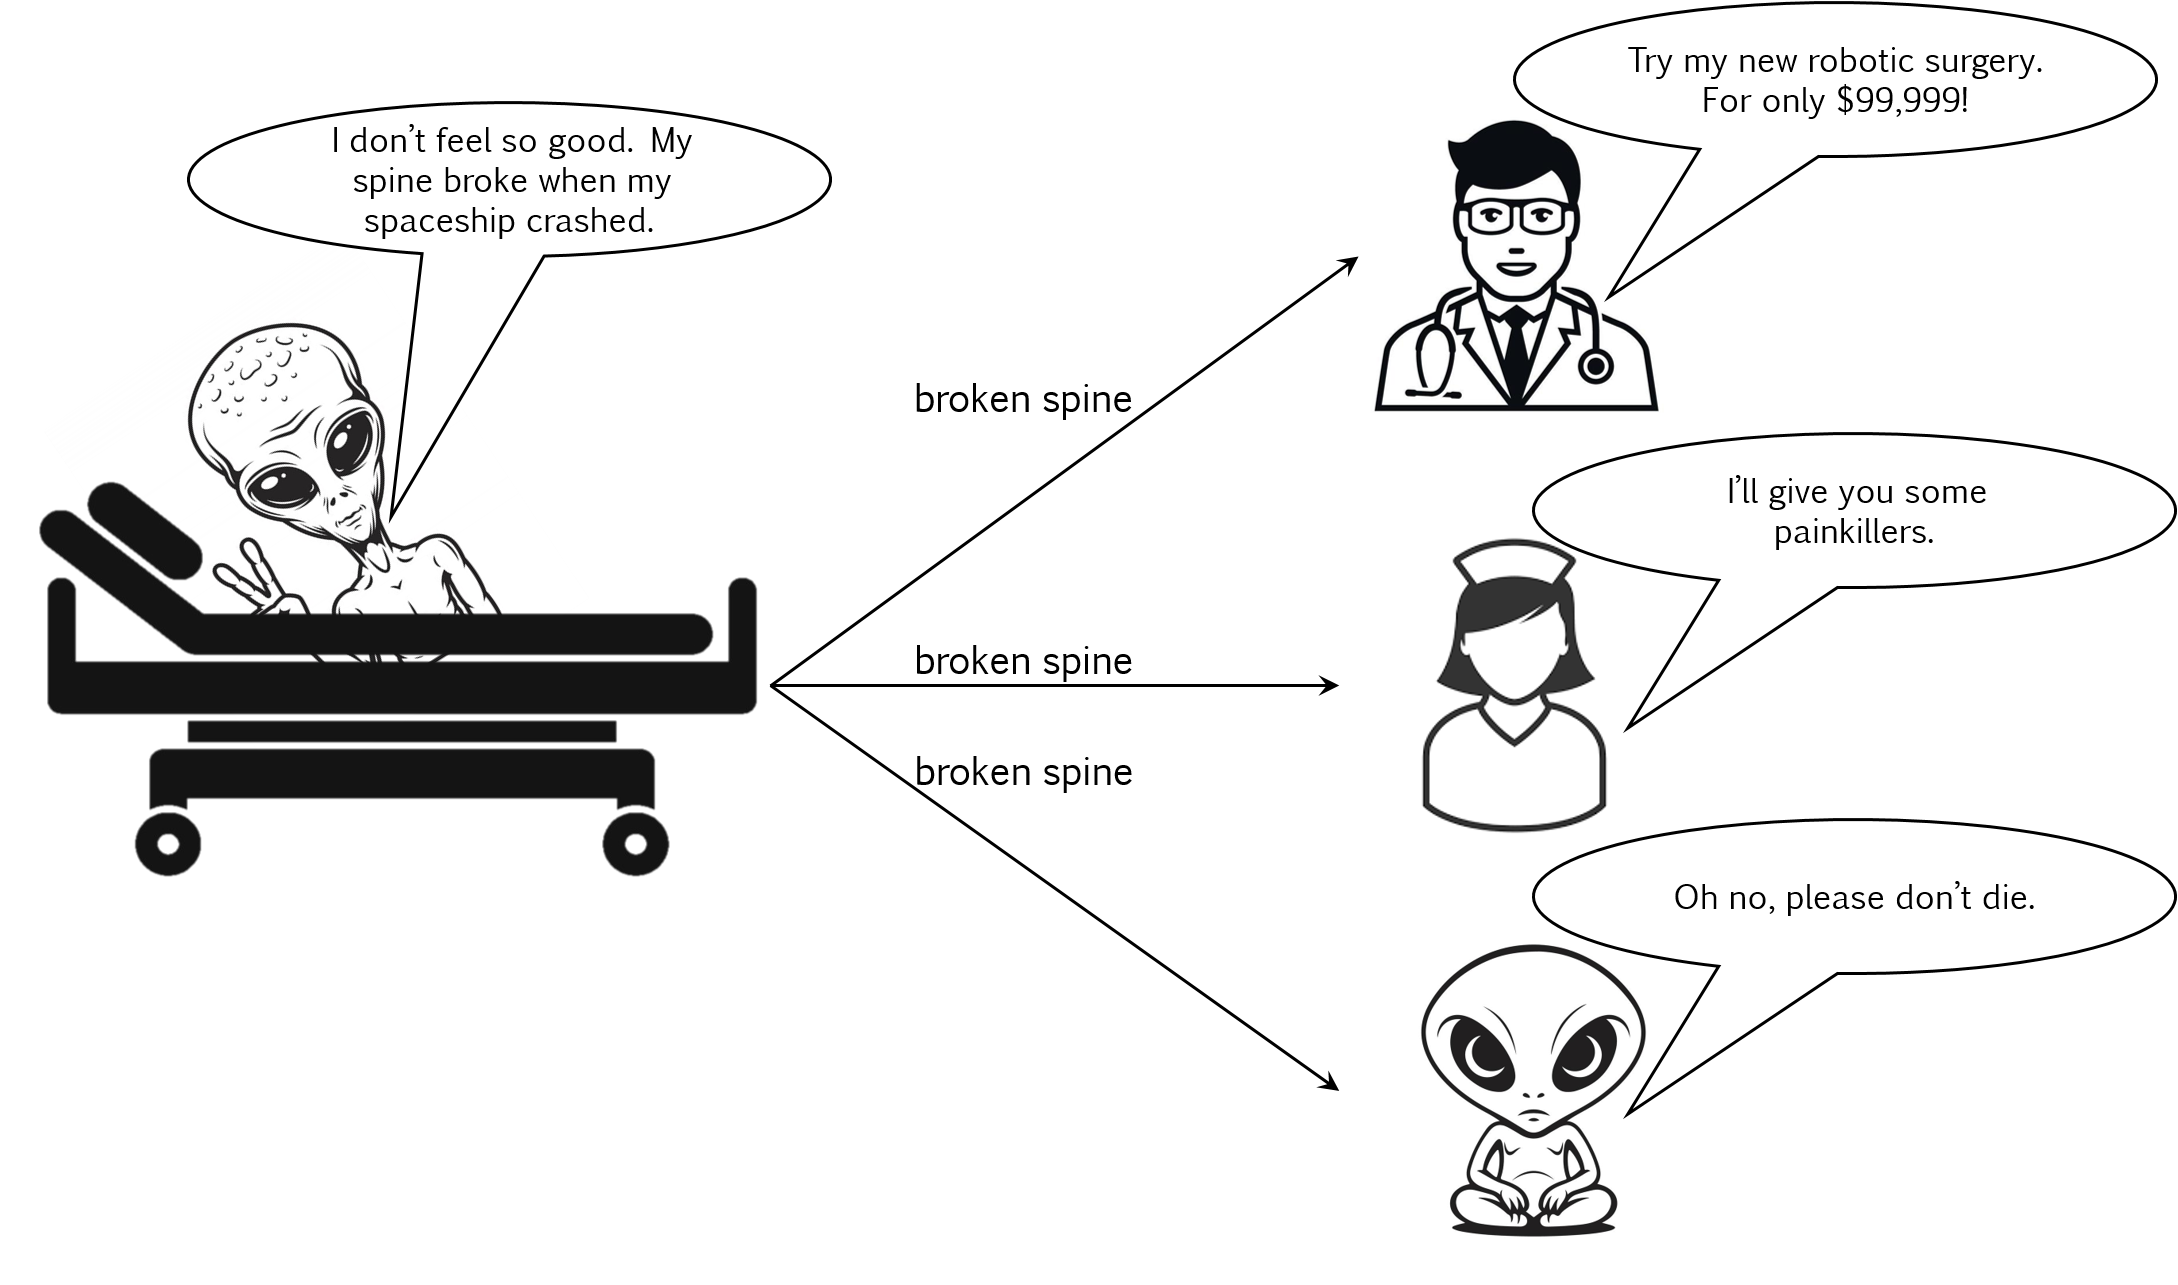
\includegraphics[width=\linewidth]{img/observer_art.png}
    %\caption{.} \label{fig:observer_alien_art}   
    \end{minipage}
    \captionof{figure}{The alien subject reports his health to the observers on the right.}

\end{tabular}

\end{table}


Let's define the classes this pattern uses:
\begin{itemize}
    \item \texttt{ISubject} -- the abstract subject (aka subject interface). Defines the abstract attach, detach and notify methods.
    \item \texttt{Subject} -- The object of interest whose internal state changes we want to observe. It maintains a list of observers and it is able to \textit{attach} an observer to it,  \textit{detach} it, or \textit{notify} all observers.  \footnote{Strictly speaking, it maintains a list of \texttt{IObserver}s and concreted observers, which inherit from \texttt{IObserver} are appended to it via the attach method. Due to polymorphism the list can accommodate all subclasses of it. Hence \texttt{IObserver} is downcast to the class of the concrete observer.} It's able to modify and return the state.
    \item \texttt{IObserver} -- the observer interface. Defines the abstract \textit{update} method. 
    \item \texttt{ConcreteObserverA}, \texttt{ConcreteObserverB}, \ldots. These subclasses of \texttt{IObserver} inherit from it and implement the update method. It's also convenient for them to store a reference to \texttt{Subject} in order to query its data if necessary.
\end{itemize}

Now whenever the state to be observed changed in the \texttt{Subject}, it is responsible to call the \texttt{notifyObservers} method inside the method itself. For example if \texttt{Subject} has a method \texttt{motifyState}, it is responsible to call \texttt{notifyObserver} in it in order to broadcast the new state to the observers.
Expressing these ideas in UML, the following diagram is constructed. In the diagram, \texttt{Subject} and \texttt{Observer} are concrete classes.

% https://www.google.com/search?sca_esv=590541752&rlz=1C1CHZO_enDE1014DE1014&sxsrf=AM9HkKl3oNStieHmmHszKxkN_ha6nbZ--A:1702474096074&q=observer+design+pattern&tbm=isch&source=lnms&sa=X&ved=2ahUKEwjl-PCdwoyDAxXZgP0HHRnSAKQQ0pQJegQIDBAB&biw=1536&bih=703&dpr=1.25#imgrc=g9PsZJCHyII2sM&imgdii=eHBzmWAfagcA8M
% wiki image
% and https://stg-tud.github.io/eise/WS14-EiSE-18-Observer_Design_Pattern.pdf

\begin{figure}[H]
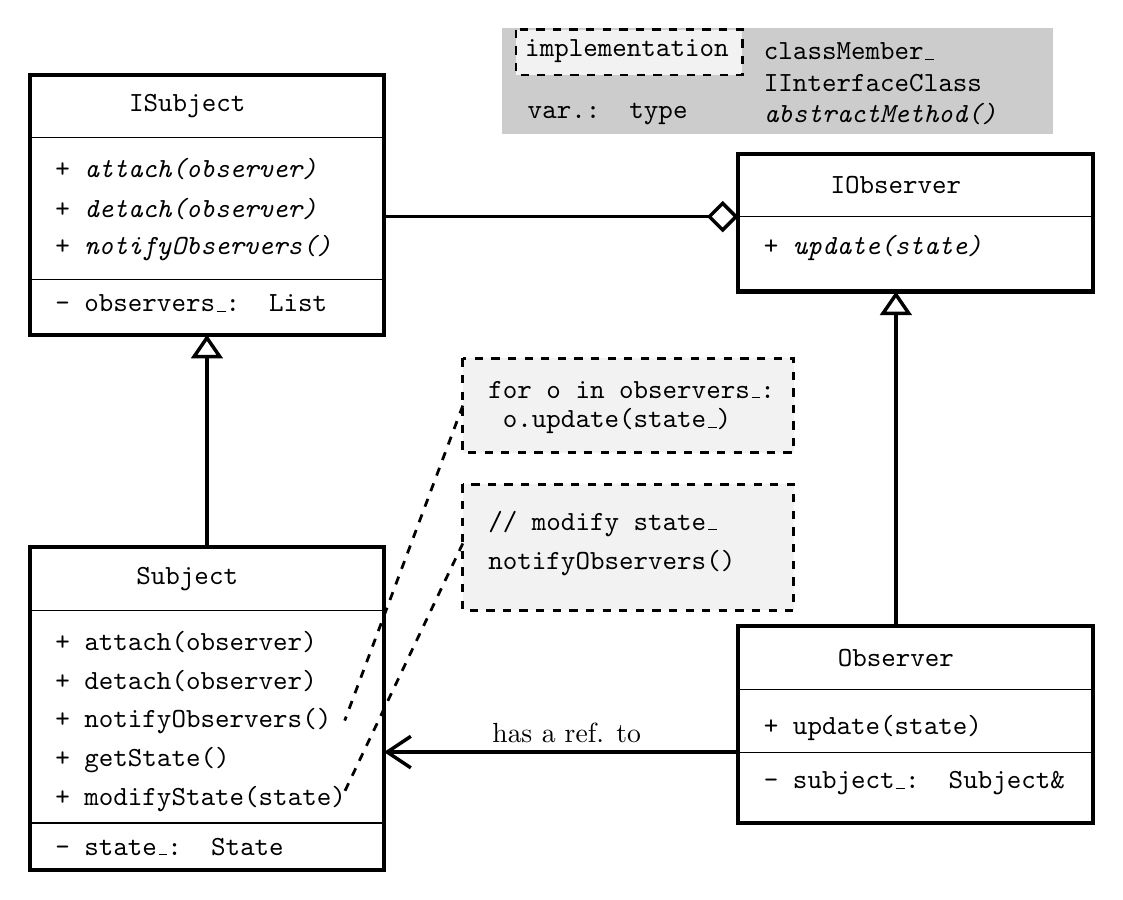
\begin{tikzpicture}
  \centering
  %--------------- Class Subject --------------- 
  \draw[line width=1.5pt] (0,-0.1) rectangle (4.5,4);
  % Class Title
  \node[align=center] at (2,3.6) {\texttt{Subject}};
  % Public Methods Section
  \draw (0,3.2) -- (4.5,3.2);
  \node[align=left,anchor=west] at (0.2,2.8) {\texttt{+ attach(observer)}};
  \node[align=left,anchor=west] at (0.2,2.3) {\texttt{+ detach(observer)}};
  \node[align=left,anchor=west] at (0.2,1.8) {\texttt{+ notifyObservers()}};
  \node[align=left,anchor=west] at (0.2,1.3) {\texttt{+ getState()}};
  \node[align=left,anchor=west] at (0.2,0.8) {\texttt{+ modifyState(state)}};
  \draw (0,0.5) -- (4.5,0.5);
  \node[align=left,anchor=west] at (0.2,0.2) {\texttt{- state\_: State}};
  %--------------- legend  --------------- 
  \fill [gray!40] (6,10.6) rectangle (13,9.25);
  \node[align=left,anchor=west] at (9.2,9.5) {\texttt{\textit{abstractMethod()}}};
  \node[align=left,anchor=west] at (9.2,9.9) {\texttt{IInterfaceClass}};
  \node[align=left,anchor=west] at (9.2,10.3) {\texttt{classMember\_}};
  \draw[line width=1pt,dashed,fill=gray!10] (6.175,10.575) rectangle (9.05,10);
  \node[align=right,anchor=east] at (9,10.3) {\texttt{implementation}};
  \node[align=left,anchor=west] at (6.2,9.5) {\texttt{var.: type}};
  %--------------- Class IObserver --------------- 
  \draw[line width=1.5pt] (9,7.25) rectangle (13.5,9);
  
  \node[align=center] at (11,8.6) {\texttt{IObserver}};
  {\texttt{Observer}};
  \draw (9,8.2) -- (13.5,8.2);
  \node[align=left,anchor=west] at (9.2,7.8) {\texttt{+ \textit{update(state)}}};
  
  
  %--------------- Class ISubject --------------- 
  \draw[line width=1.5pt] (0,6.7) rectangle (4.5,10);
  \node[align=center] at (2,9.6) {\texttt{ISubject}};
  % Public Methods Section
  \draw (0,9.2) -- (4.5,9.2);
  \node[align=left,anchor=west] at (0.2,8.8) {\texttt{+ \textit{attach(observer)}}};
  \node[align=left,anchor=west] at (0.2,8.3) {\texttt{+ \textit{detach(observer)}}};
  \node[align=left,anchor=west] at (0.2,7.8) {\texttt{+ \textit{notifyObservers()}}};
  \draw (0,7.4) -- (4.5,7.4);
  \node[align=left,anchor=west] at (0.2,7.1) {\texttt{- observers\_: List}};
  
  %---------------  notifyObservers method --------------- 
  % (4.5 + d, 6.7-d)
  \draw[line width=1pt,dashed,fill=gray!10] (5.5,6.4) rectangle (9.7,5.2);
  \node[align=left,anchor=west] at (5.7,6) {\texttt{for o in observers\_:}};
  \node[align=left,anchor=west] at (5.7,5.6) {\texttt{ 
 o.update(state\_)}};

 %---------------  modifyState method --------------- 
  % (4.5 + d, 6.7-d)
  \draw[line width=1pt,dashed,fill=gray!10] (5.5,4.8) rectangle (9.7,3.2);
  \node[align=left,anchor=west] at (5.7,4.3) {\texttt{// modify state\_}};
  \node[align=left,anchor=west] at (5.7,3.8) {\texttt{notifyObservers()}};
  %--------------- Class Observer --------------- 
  \draw[line width=1.5pt] (9,0.5) rectangle (13.5,3);
  \node[align=center] at (11,2.6) {\texttt{Observer}};
  \draw (9,2.2) -- (13.5,2.2);
  \node[align=left,anchor=west] at (9.2,1.7) {\texttt{+ update(state)}};
  \draw (9,1.4) -- (13.5,1.4);
  \node[align=left,anchor=west] at (9.2,1.0) {\texttt{- subject\_: Subject\&}};

  %--------------- arrows --------------- 
  %(5.4,2.25) -> (2.25,6.7)
  \draw[-{Triangle[open, fill=white, length=3mm, width=4mm]}, line width=1.25pt]  (2.25,4) -- (2.25,6.7);
  % Obs -> Sub
  \draw[-{Straight Barb[open, fill=white, length=3mm, width=4mm]}, line width=1.25pt]  (9,1.4) -> (4.5,1.4);
  \node[align=left,anchor=west] at (5.75,1.65) {has a ref. to};
  % ISub -> Iob
  \draw[-{Diamond[open, fill=white, length=4mm, width=4mm]}, line width=1.25pt] (4.5,8.2) -- (9,8.2);
  % Ob -> IOb
  \draw[-{Triangle[open, fill=white, length=3mm, width=4mm]}, line width=1.25pt] (11,3) -- (11,7.25);
  % implementation -> modifyState 
  \draw[-, line width=1pt, dashed]  (5.5,4.05) -- (4.0,0.9);
  % implementation -> notifyObservers 
  \draw[-, line width=1pt, dashed]  (5.5, 5.8) -- (4.0,1.8) ;
\end{tikzpicture}
\caption{UML diagram of the observer design pattern.} \label{fig:observer_uml}
\end{figure}

A practical example that demonstrates the observer design pattern is a model of the stock market found in \ref{app:obs_stock_market}.

A \texttt{StockMarket} subject calls \texttt{UpdateState()} to update its ticker (fancy word for stock symbol) pairs modelled by the state variable \texttt{pairs\_}. The latter stores the price for each stock marker symbol in a dictionary, e.g. \texttt{\{\{GOOG: 152.99\}, \{NVDA: 461.72\}\}}. \texttt{UpdateState()} furthermore calls \texttt{NotifyObservers()}, which in turns goes through all observers and for each pair in \texttt{pairs\_} it calls \texttt{Update(std::string ticker, double price)}. \texttt{ticker} is the first field of each pair and \texttt{price} its second. \texttt{Investor} is a dummy concrete observer but bot keeps a history of each pair in its internal variables, e.g. \texttt{GOOG: [148, 152, 149]} hence can perform a simulation of an analysis.

Table \ref{tab:obs_uml_to_stock_market_code} shows how the diagram in Fig. \ref{fig:observer_uml} corresponds to the stock market code in \ref{app:obs_stock_market}.
\begin{table}[H]
  \centering
  \begin{tabular}{p{0.15\linewidth}|p{0.22\linewidth}||p{0.22\linewidth}|p{0.29\linewidth}}
    \textbf{Diagram} & \textbf{Code} & \textbf{Diagram} & \textbf{Code} \\
    \midrule
      \texttt{Subject} & \texttt{StockMarket} & \texttt{attach} & \texttt{AttachObserver} \\
      \texttt{detach} & \texttt{DetachObserver} & \texttt{update(state)} & \texttt{Update(std::string, int)} \\
      \texttt{state\_} & \texttt{pairs\_} & \texttt{modifyState} & \texttt{UpdatePrices} \\
      \texttt{getState()} & \texttt{pairs()} & \texttt{ConcreteObserver} & \texttt{Bot}, \texttt{Investor} \\
    \hline
  \end{tabular}
  \caption{How the naming in Fig. \ref{fig:observer_uml} corresponds to that in \ref{app:obs_stock_market}'s code.} \label{tab:obs_uml_to_stock_market_code}
\end{table}

In the end, the two observers report their updates and the bot additionally makes its super sophisticated and advanced analysis.
\begin{verbatim}
-------- day 15 --------
  Investor Alice received update: AAPL price is 183.4
  Investor Alice received update: NVDA price is 477.4
  Investor Alice received update: GOOG price is 154.3
  Bot received an update of 183.4 on AAPL ticker
  Bot received an update of 477.4 on NVDA ticker
  Bot received an update of 154.3 on GOOG ticker
  Bot says: AAPL's tomorrow price will be 189.28 with RSI = 72 --> SELL
  Bot says: NVDA's tomorrow price will be 476.77 with RSI = 68 --> HOLD
  Bot says: GOOG's tomorrow price will be 163.90 with RSI = 24 --> BUY
\end{verbatim}





% https://stg-tud.github.io/eise/WS14-EiSE-18-Observer_Design_Pattern.pdf

\subsection{Other Design Patterns}


%=-=-=-=-=-=-=-=-=-=-=-=-=-=-=-=-=-=-=-=-=-=-=-=-=-=-=-=-=-=-=-=-=-=-=-=-=-=-=-=-
% References
%=-=-=-=-=-=-=-=-=-=-=-=-=-=-=-=-=-=-=-=-=-=-=-=-=-=-=-=-=-=-=-=-=-=-=-=-=-=-=-=-
\newpage
\printbibliography



%=-=-=-=-=-=-=-=-=-=-=-=-=-=-=-=-=-=-=-=-=-=-=-=-=-=-=-=-=-=-=-=-=-=-=-=-=-=-=-=-
% Appendices
%=-=-=-=-=-=-=-=-=-=-=-=-=-=-=-=-=-=-=-=-=-=-=-=-=-=-=-=-=-=-=-=-=-=-=-=-=-=-=-=-
\newpage
\appendix

\section{Appendices}

% ------------------------ New appendix ------------------------ %
\newpage
\subsection{Observer: stock market model}
\label{app:obs_stock_market}

\lstinputlisting[language=c++,caption={A stock market system modelled by the observer design apttern (\detokenize{src/observer.cpp)}.}, label=src:observerstockmarket]{src/observer.cpp}



\end{document}
